\def\topic{Sorting}
\input{comp125lectureHeader}

\section{Overview}

\begin{figure}
\centering	
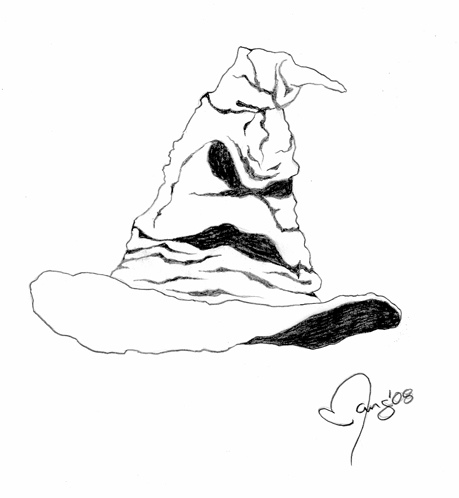
\includegraphics[width=.4\textwidth]{images/sortingHat.jpg}
\caption{Art: Nancy Hebert, licensed for reuse.}
\end{figure}

  We explore the two standard sorting algorithms - insertion, and selection, along with analysis of the two. In addition, we also take a less detailed look at merge sort.
 
\subsection{Why is sorting important?}

Sorting a collection makes it easy to analyse data. Several tasks are made simpler if a collection is sorted, such as:

\begin{itemize}
\item finding the lowest value (first value in a collection sorted in ascending order)
\item finding the highest value (last value in a collection sorted in ascending order)
\item finding the median value (item at \texttt{arr.length/2})
\item checking if the array contains any negative value (it does if the lowest value is less than zero)	
\item checking if the array contains only negative value (it does if the highest value is less than zero)
\item faster search (using binary search algorithm)	
\end{itemize}

\newcommand{\selunsorted}{{80,70,10,10,50,30,90,40}}
\newcommand{\selitera}{{10,70,80,10,50,30,90,40}}
\newcommand{\seliterb}{{10,10,80,70,50,30,90,40}}
\newcommand{\seliterc}{{10,10,30,70,50,80,90,40}}
\newcommand{\seliterd}{{10,10,30,40,50,80,90,70}}
\newcommand{\selitere}{{10,10,30,40,50,80,90,70}}
\newcommand{\seliterf}{{10,10,30,40,50,70,90,80}}
\newcommand{\seliterg}{{10,10,30,40,50,70,80,90}}
\newcommand{\selsorted}{{10,10,30,40,50,70,80,90}}
\tikzstyle{unsorted} = [draw,fill=red!40,minimum size=3.6em]
\tikzstyle{sorted} = [draw,fill=green!90!black,minimum size=3.6em]
\begin{tikzpicture}
\foreach \x in {0,1,...,7} {
	\node[unsorted] at (\x*1.8,5) (block\x) {\pgfmathparse{\selunsorted[\x]}\pgfmathresult};
	\node at (\x*1.8, 4) {a[\x]};
	
	\node[sorted] at (\x*1.8,1) (block\x) {\pgfmathparse{\selsorted[\x]}\pgfmathresult};
	\node at (\x*1.8, 0) {a[\x]};	
}
	\draw [line width=3mm, ->, black!80!white] (6.2,3.5) -- (6.2, 2);
\end{tikzpicture}

\section{Selection Sort}

The principle behind selection sort is:

\begin{center}
	\emph{
		Swap the smallest item in the unsorted part of the array with the first item of the unsorted part of the array}
\end{center}

\tikzstyle{unsorted} = [draw,fill=red!40,minimum size=2.4em]
\tikzstyle{sorted} = [draw,fill=green!90!black,minimum size=2.4em]
\tikzstyle{current} = [draw,fill=red,minimum size=3em]

\bgroup \tikzset{png export} \begin{tikzpicture}
\pgfmathsetmacro{\step}{15}
\pgfmathsetmacro{\headerChange}{1}
\pgfmathsetmacro{\change}{-2}


\foreach \x in {0,1,...,7} {
	\ifthenelse{\x=0}
	{
	\node[current] at (\x*1.5,\step) (block\x) {\pgfmathparse{\selunsorted[\x]}\pgfmathresult};
	}
	{
	\node[unsorted] at (\x*1.5,\step) (block\x) {\pgfmathparse{\selunsorted[\x]}\pgfmathresult};
	}
	\node at (\x*1.5, \step+\headerChange) {a[\x]};
}
\draw [ultra thick, rounded corners, <->] (0*1.5, \step-0.6) -- (0*1.5, \step-1) -- (2*1.5, \step-1) -- (2*1.5, \step-0.5);

\edef\step{\step+\change}
\node[sorted] at (0*1.5,\step) (block0) {\pgfmathparse{\selitera[0]}\pgfmathresult};

\foreach \x in {1,...,7} {
	\ifthenelse{\x=1}
	{
		\node[current] at (\x*1.5,\step) (block\x) {\pgfmathparse{\selitera[\x]}\pgfmathresult};
	}
	{
	\node[unsorted] at (\x*1.5,\step) (block\x) {\pgfmathparse{\selitera[\x]}\pgfmathresult};
	}
}
\draw [ultra thick, rounded corners, <->] (1*1.5, \step-0.6) -- (1*1.5, \step-1) -- (3*1.5, \step-1) -- (3*1.5, \step-0.5);

\edef\step{\step+\change}
\foreach \x in {0,...,1} {
	\node[sorted] at (\x*1.5,\step) (block\x) {\pgfmathparse{\seliterb[\x]}\pgfmathresult};
}
\foreach \x in {2,...,7} {
	\ifthenelse{\x=2}
	{
		\node[current] at (\x*1.5,\step) (block\x) {\pgfmathparse{\seliterb[\x]}\pgfmathresult};
		}
		{
		\node[unsorted] at (\x*1.5,\step) (block\x) {\pgfmathparse{\seliterb[\x]}\pgfmathresult};

		}
}
\draw [ultra thick, rounded corners, <->] (2*1.5, \step-0.6) -- (2*1.5, \step-1) -- (5*1.5, \step-1) -- (5*1.5, \step-0.5);

\edef\step{\step+\change}
\foreach \x in {0,...,2} {
	\node[sorted] at (\x*1.5,\step) (block\x) {\pgfmathparse{\seliterc[\x]}\pgfmathresult};
}
\foreach \x in {3,...,7} {
	\ifthenelse{\x=3} {
	\node[current] at (\x*1.5,\step) (block\x) {\pgfmathparse{\seliterc[\x]}\pgfmathresult};
	}
	{
	\node[unsorted] at (\x*1.5,\step) (block\x) {\pgfmathparse{\seliterc[\x]}\pgfmathresult};
	}
}
\draw [ultra thick, rounded corners, <->] (3*1.5, \step-0.6) -- (3*1.5, \step-1) -- (7*1.5, \step-1) -- (7*1.5, \step-0.5);

\edef\step{\step+\change}
\foreach \x in {0,...,3} {
	\node[sorted] at (\x*1.5,\step) (block\x) {\pgfmathparse{\seliterd[\x]}\pgfmathresult};
}
\foreach \x in {4,...,7} {
	\ifthenelse{\x=4}
	{
	\node[current] at (\x*1.5,\step) (block\x) {\pgfmathparse{\seliterd[\x]}\pgfmathresult};
	}
	{
	\node[unsorted] at (\x*1.5,\step) (block\x) {\pgfmathparse{\seliterd[\x]}\pgfmathresult};
	}
}
\draw [ultra thick, rounded corners, <->] (4*1.5-0.2, \step-0.6) -- (4*1.5-0.2, \step-1) -- (4*1.5+0.2, \step-1) -- (4*1.5+0.2, \step-0.6);

\edef\step{\step+\change}
\foreach \x in {0,...,4} {
	\node[sorted] at (\x*1.5,\step) (block\x) {\pgfmathparse{\selitere[\x]}\pgfmathresult};
}
\foreach \x in {5,...,7} {
	\ifthenelse{\x=5} 
	{
	\node[current] at (\x*1.5,\step) (block\x) {\pgfmathparse{\selitere[\x]}\pgfmathresult};
	}
	{
	\node[unsorted] at (\x*1.5,\step) (block\x) {\pgfmathparse{\selitere[\x]}\pgfmathresult};
	}
}
\draw [ultra thick, rounded corners, <->] (5*1.5, \step-0.6) -- (5*1.5, \step-1) -- (7*1.5, \step-1) -- (7*1.5, \step-0.5);

\edef\step{\step+\change}
\foreach \x in {0,...,5} {
	\node[sorted] at (\x*1.5,\step) (block\x) {\pgfmathparse{\seliterf[\x]}\pgfmathresult};
}
\foreach \x in {6,...,7} {
	\ifthenelse{\x=6}
	{
	\node[current] at (\x*1.5,\step) (block\x) {\pgfmathparse{\seliterf[\x]}\pgfmathresult};
	}
	{
	\node[unsorted] at (\x*1.5,\step) (block\x) {\pgfmathparse{\seliterf[\x]}\pgfmathresult};
	}
}
\draw [ultra thick, rounded corners, <->] (6*1.5, \step-0.6) -- (6*1.5, \step-1) -- (7*1.5, \step-1) -- (7*1.5, \step-0.5);

\edef\step{\step+\change}
\foreach \x in {0,...,6} {
	\node[sorted] at (\x*1.5,\step) (block\x) {\pgfmathparse{\seliterg[\x]}\pgfmathresult};
}
\foreach \x in {7,...,7} {
	\node[unsorted] at (\x*1.5,\step) (block\x) {\pgfmathparse{\seliterg[\x]}\pgfmathresult};
}

\foreach \x in {0,1,...,7} {
	\node[sorted] at (\x*1.5,\step) (block\x) {\pgfmathparse{\selsorted[\x]}\pgfmathresult};
}
\end{tikzpicture} \egroup

\subsection{Selection Sort sample pseudo-code}

\IncMargin{1em}
\begin{algorithm}[H]
	\SetAlgoLined
\KwData{\texttt{int[] arr}}
\KwResult{none (array is sorted in ascending order at the end)}
set \texttt{i} to 0\;
\While{\texttt{i} is not the last index}{
	set \texttt{minIndex} to \texttt{i}\;
	set \texttt{k} to \texttt{i+1}\;
	\While{\texttt{k} is a valid index} {
		\If{item at index \texttt{k} < item at index \texttt{minIndex}}{
			update \texttt{minIndex} to hold value of \texttt{k}\;
		}
	}
	swap item at index \texttt{minIndex} with item at index \texttt{i}\;
}
\caption{Selection Sort \label{selectionsort}}
\end{algorithm}

\newpage
\subsection{Selection Sort sample source code}

\begin{lstlisting}[basicstyle=\small]
//helper 1
public static void swap(int[] a, int idx1, int idx2) {
	if(a == null) nothing to do 
		return;
	if(idx1 < 0 || idx1 >= a.length) //invalid index 1
		return;
	if(idx2 < 0 || idx2 >= a.length) //invalid index 2
		return;
	int temp = a[idx1];
	a[idx1] = a[idx2];
	a[idx2] = temp;
}

//helper 2
public static int indexSmallestItem(int[] a, int start) {
	if(a == null) 
		return -1; //error code
	if(start < 0 || start >= a.length) //invalid index
		return -1;
	int result = start; 
	for(int k=start+1; k < a.length; k++) {
		if(a[k] < a[result]) {
			result = k;
		}
	}
	return result;
}

//sorting method
public static void selectionSort(int[] arr) {
	if(arr == null) //nothing to do
		return;
	for(int i=0; i < arr.length - 1; i++) {
		int minIndex = indexSmallestItem(arr, i);	
		swap(arr, i, minIndex);
	}
}
\end{lstlisting}

\newpage
The helpers can be written inline as well, with which the method is:

\begin{lstlisting}
	//sorting method
public static void selectionSort(int[] arr) {
	if(arr == null) //nothing to do
		return;
	for(int i=0; i < arr.length - 1; i++) {
		int minIndex = i;
		for(int k=i+1; k < arr.length; k++) {
			if(arr[k] < arr[minIndex]) {
				minIndex = k;
			}
		}
		int temp = arr[i];
		arr[i] = arr[minIndex];
		arr[minIndex] = temp;
	}
}
\end{lstlisting}

\begin{exercise}[8][Trace selection sort execution]
Trace the status of the array at the end of each iteration of the loop controlled by variable \texttt{i} in selection sort for the following cases:

\begin{enumerate}
\item \texttt{arr = \{4, 3, 6, 5, 2, 1\}}
\item \texttt{arr = \{1, 8, 2, 7, 3, 6\}}
\end{enumerate}
\end{exercise}

\begin{answer}
\begin{enumerate}
\item 
\begin{verbatim}
4 3 6 5 2 1
1 3 6 5 2 4
1 2 6 5 3 4
1 2 3 5 6 4
1 2 3 4 6 5
1 2 3 4 5 6	
\end{verbatim}

\item 
\begin{verbatim}
1 8 2 7 3 6
1 8 2 7 3 6 (no change as smallest item already at front)
1 2 8 7 3 6
1 2 3 7 8 6
1 2 3 6 8 7
1 2 3 6 7 8
\end{verbatim}
\end{enumerate}
\end{answer}

	\newpage

\subsection{Sorting array of objects}

Since objects cannot be compared using the primitive comparison operators ($>, <, \geq, \leq$), we must use the method \texttt{compareTo} to compare them.

Essentially, 

\begin{lstlisting}
obj1 < obj2
//is same as
obj1.compareTo(obj2) == -1
\end{lstlisting}

Similarly, 

\begin{lstlisting}
obj1 > obj2
//is same as
obj1.compareTo(obj2) == 1
\end{lstlisting}

The only two statements in the sorted algorithm that are affected are:

\begin{lstlisting}
if(arr[k] < arr[minIndex]) //on line 8
int temp = arr[i]; //on line 12
\end{lstlisting}

The sorting algorithm applied on array of objects changes to:

\begin{lstlisting}[style=buggy]
//sorting method
public static void selectionSort(Circle[] arr) {
	if(arr == null) //nothing to do
		return;
	for(int i=0; i < arr.length - 1; i++) {
		int minIndex = i;
		for(int k=i+1; k < arr.length; k++) {
			if(@arr[k].compareTo(arr[minIndex]) == -1@) {
				minIndex = k;
			}
		}
		@Circle temp = arr[i];@
		arr[i] = arr[minIndex];
		arr[minIndex] = temp;
	}
}
\end{lstlisting}

\newpage

\subsection{Variations to sorting algorithm}

Sometimes, the basis of sorting might be a bit more complex than simple numerical comparison. For example, I might want to sort an array of integers in ascending order of number of divisors. For example, if the array is \texttt{\{14, 5202, 12, 121, 36\}}, the diferent states of the array sorted on different criteria are below:

\begin{enumerate}
\item Based on numerical value: \texttt{\{12, 14, 36, 121, 5202\}}	
\item Based on number of digits: \texttt{\{14, 12,  36, 121, 5202\}}	
\item Based on number of divisors: \texttt{\{121, 5202, 14, 12, 36\}}	
\end{enumerate}

This \textbf{only} affects the comparison statement.

In each of the above situations, the comparison statements would be:

\begin{enumerate}
\item Based on numerical value: 
\begin{lstlisting}
if(arr[k] < arr[minIndex])
\end{lstlisting}
\item Based on number of digits: 
\begin{lstlisting}
if(nDigits(arr[k]) < nDigits(arr[minIndex]))
\end{lstlisting}
\item Based on number of divisors:
\begin{lstlisting}
if(nDivisors(arr[k]) < nDivisors(arr[minIndex]))
\end{lstlisting}
\end{enumerate}

In general, when comparing on a function of the items of the array, we should be using,

\begin{lstlisting}
if(someFunction(arr[k]) < someFunction(arr[minIndex]))
\end{lstlisting}

Where the simplest function is the identity function (the item itself), reducing the statement to,

\begin{lstlisting}
if(arr[k] < arr[minIndex])
\end{lstlisting}

\section{Insertion Sort}

The principle behind insertion sort is:

\begin{center}
	\emph{
		Put the first item of the unsorted part at the right place in the sorted part.
	}
\end{center}

\subsection*{Example 1}
\newcommand{\insunsorted}{{80,70,10,10,50,30,90,40}}
\newcommand{\insitera}{{70,80,10,10,50,30,90,40}}
\newcommand{\insiterb}{{10,70,80,10,50,30,90,40}}
\newcommand{\insiterc}{{10,10,70,80,50,30,90,40}}
\newcommand{\insiterd}{{10,10,50,70,80,30,90,40}}
\newcommand{\insitere}{{10,10,30,50,70,80,90,40}}
\newcommand{\insiterf}{{10,10,30,50,70,80,90,40}}
\newcommand{\insiterg}{{10,10,30,40,50,70,80,90}}
\newcommand{\inssorted}{{10,10,30,40,50,70,80,90}}
\begin{center}
\begin{tikzpicture}[scale = 0.8]
\pgfmathsetmacro{\step}{15}
\pgfmathsetmacro{\headerChange}{1}
\pgfmathsetmacro{\change}{-2}

\foreach \x in {0,...,0} {
	\node[sorted] at (\x*1.5,\step) (block\x) {\pgfmathparse{\insunsorted[\x]}\pgfmathresult};
}
\node at (0, \step+\headerChange) {a[0]};
\foreach \x in {1,...,7} {
	\ifthenelse{\x=1}
	{
	\node[current] at (\x*1.5,\step) (block\x) {\pgfmathparse{\insunsorted[\x]}\pgfmathresult};
	}
	{
	\node[unsorted] at (\x*1.5,\step) (block\x) {\pgfmathparse{\insunsorted[\x]}\pgfmathresult};
	}
	\node at (\x*1.5, \step+\headerChange) {a[\x]};
}
\draw [ultra thick, rounded corners, ->] (1*1.5, \step-0.6) -- (1*1.5, \step-1) -- (-0.75, \step-1) -- (-0.75, \step-0.5);

\edef\step{\step+\change}
\node[sorted] at (0*1.5,\step) (block0) {\pgfmathparse{\insitera[0]}\pgfmathresult};

\foreach \x in {0,...,1} {
	\node[sorted] at (\x*1.5,\step) (block\x) {\pgfmathparse{\insitera[\x]}\pgfmathresult};
}
\foreach \x in {2,...,7} {
	\ifthenelse{\x=2}
	{
		\node[current] at (\x*1.5,\step) (block\x) {\pgfmathparse{\insitera[\x]}\pgfmathresult};
	}
	{
	\node[unsorted] at (\x*1.5,\step) (block\x) {\pgfmathparse{\insitera[\x]}\pgfmathresult};
	}
}
\draw [ultra thick, rounded corners, ->] (2*1.5, \step-0.6) -- (2*1.5, \step-1) -- (-0.75, \step-1) -- (-0.75, \step-0.5);

\edef\step{\step+\change}
\foreach \x in {0,...,2} {
	\node[sorted] at (\x*1.5,\step) (block\x) {\pgfmathparse{\insiterb[\x]}\pgfmathresult};
}
\foreach \x in {3,...,7} {
	\ifthenelse{\x=3}
	{
		\node[current] at (\x*1.5,\step) (block\x) {\pgfmathparse{\insiterb[\x]}\pgfmathresult};
		}
		{
		\node[unsorted] at (\x*1.5,\step) (block\x) {\pgfmathparse{\insiterb[\x]}\pgfmathresult};

		}
}
\draw [ultra thick, rounded corners, ->] (3*1.5, \step-0.6) -- (3*1.5, \step-1) -- (-0.75 + 1*1.5, \step-1) -- (-0.75 + 1*1.5, \step-0.5);

\edef\step{\step+\change}
\foreach \x in {0,...,3} {
	\node[sorted] at (\x*1.5,\step) (block\x) {\pgfmathparse{\insiterc[\x]}\pgfmathresult};
}
\foreach \x in {4,...,7} {
	\ifthenelse{\x=4} {
	\node[current] at (\x*1.5,\step) (block\x) {\pgfmathparse{\insiterc[\x]}\pgfmathresult};
	}
	{
	\node[unsorted] at (\x*1.5,\step) (block\x) {\pgfmathparse{\insiterc[\x]}\pgfmathresult};
	}
}
\draw [ultra thick, rounded corners, ->] (4*1.5, \step-0.6) -- (4*1.5, \step-1) -- (-0.75 + 2*1.5, \step-1) -- (-0.75 + 2*1.5, \step-0.5);

\edef\step{\step+\change}
\foreach \x in {0,...,4} {
	\node[sorted] at (\x*1.5,\step) (block\x) {\pgfmathparse{\insiterd[\x]}\pgfmathresult};
}
\foreach \x in {5,...,7} {
	\ifthenelse{\x=5}
	{
	\node[current] at (\x*1.5,\step) (block\x) {\pgfmathparse{\insiterd[\x]}\pgfmathresult};
	}
	{
	\node[unsorted] at (\x*1.5,\step) (block\x) {\pgfmathparse{\insiterd[\x]}\pgfmathresult};
	}
}
\draw [ultra thick, rounded corners, ->] (5*1.5, \step-0.6) -- (5*1.5, \step-1) -- (-0.75 + 2*1.5, \step-1) -- (-0.75 + 2*1.5, \step-0.5);

\edef\step{\step+\change}
\foreach \x in {0,...,5} {
	\node[sorted] at (\x*1.5,\step) (block\x) {\pgfmathparse{\insitere[\x]}\pgfmathresult};
}
\foreach \x in {6,...,7} {
	\ifthenelse{\x=6} 
	{
	\node[current] at (\x*1.5,\step) (block\x) {\pgfmathparse{\insitere[\x]}\pgfmathresult};
	}
	{
	\node[unsorted] at (\x*1.5,\step) (block\x) {\pgfmathparse{\insitere[\x]}\pgfmathresult};
	}
}
\draw [ultra thick, rounded corners, ->] (6*1.5, \step-0.6) -- (6*1.5, \step-1) -- (6*1.5-0.75, \step-1) -- (6*1.5-0.75, \step-0.6);

\edef\step{\step+\change}
\foreach \x in {0,...,6} {
	\node[sorted] at (\x*1.5,\step) (block\x) {\pgfmathparse{\insiterf[\x]}\pgfmathresult};
}
\foreach \x in {7,...,7} {
	\ifthenelse{\x=7}
	{
	\node[current] at (\x*1.5,\step) (block\x) {\pgfmathparse{\insiterf[\x]}\pgfmathresult};
	}
	{
	\node[unsorted] at (\x*1.5,\step) (block\x) {\pgfmathparse{\insiterf[\x]}\pgfmathresult};
	}
}
\draw [ultra thick, rounded corners, ->] (7*1.5, \step-0.6) -- (7*1.5, \step-1) -- (-0.75 + 3*1.5, \step-1) -- (-0.75 + 3*1.5, \step-0.5);

\edef\step{\step+\change}
\foreach \x in {0,...,6} {
	\node[sorted] at (\x*1.5,\step) (block\x) {\pgfmathparse{\insiterg[\x]}\pgfmathresult};
}
\foreach \x in {7,...,7} {
	\node[unsorted] at (\x*1.5,\step) (block\x) {\pgfmathparse{\insiterg[\x]}\pgfmathresult};
}

\foreach \x in {0,1,...,7} {
	\node[sorted] at (\x*1.5,\step) (block\x) {\pgfmathparse{\inssorted[\x]}\pgfmathresult};
}
\end{tikzpicture}
\end{center}


\subsection*{Example 2}
\newcommand{\inssunsorted}{{"hello", "how", "is", "everyone"}}
\newcommand{\inssitera}{{"how", "hello", "is", "everyone"}}
\newcommand{\inssiterb}{{"is", "how", "hello", "everyone"}}
\newcommand{\inssiterc}{{"is", "how", "hello", "everyone"}}
\newcommand{\insssorted}{{"is", "how", "hello", "everyone"}}
\begin{tikzpicture}
\pgfmathsetmacro{\step}{15}
\pgfmathsetmacro{\headerChange}{1}
\pgfmathsetmacro{\change}{-2}

\foreach \x in {0,...,0} {
	\node[sorted] at (\x*3,\step) (block\x) {\pgfmathparse{\inssunsorted[\x]}\pgfmathresult};
}
\node at (0, \step+\headerChange) {a[0]};
\foreach \x in {1,...,3} {
	\ifthenelse{\x=1}
	{
	\node[current] at (\x*3,\step) (block\x) {\pgfmathparse{\inssunsorted[\x]}\pgfmathresult};
	}
	{
	\node[unsorted] at (\x*3,\step) (block\x) {\pgfmathparse{\inssunsorted[\x]}\pgfmathresult};
	}
	\node at (\x*3, \step+\headerChange) {a[\x]};
}
\draw [ultra thick, rounded corners, ->] (1*3, \step-0.6) -- (1*3, \step-1) -- (-0.75, \step-1) -- (-0.75, \step-0.5);

\edef\step{\step+\change}
\node[sorted] at (0*3,\step) (block0) {\pgfmathparse{\inssitera[0]}\pgfmathresult};

\foreach \x in {0,...,1} {
	\node[sorted] at (\x*3,\step) (block\x) {\pgfmathparse{\inssitera[\x]}\pgfmathresult};
}
\foreach \x in {2,...,3} {
	\ifthenelse{\x=2}
	{
		\node[current] at (\x*3,\step) (block\x) {\pgfmathparse{\inssitera[\x]}\pgfmathresult};
	}
	{
	\node[unsorted] at (\x*3,\step) (block\x) {\pgfmathparse{\inssitera[\x]}\pgfmathresult};
	}
}
\draw [ultra thick, rounded corners, ->] (2*3, \step-0.6) -- (2*3, \step-1) -- (-0.75, \step-1) -- (-0.75, \step-0.5);

\edef\step{\step+\change}
\foreach \x in {0,...,2} {
	\node[sorted] at (\x*3,\step) (block\x) {\pgfmathparse{\inssiterb[\x]}\pgfmathresult};
}
\foreach \x in {3,...,3} {
	\ifthenelse{\x=3}
	{
		\node[current] at (\x*3,\step) (block\x) {\pgfmathparse{\inssiterb[\x]}\pgfmathresult};
		}
		{
		\node[unsorted] at (\x*3,\step) (block\x) {\pgfmathparse{\inssiterb[\x]}\pgfmathresult};

		}
}
\draw [ultra thick, rounded corners, ->] (3*3, \step-0.6) -- (3*3, \step-1) -- (3*3 - 1.5, \step-1) -- (3*3 - 1.5, \step-0.6);

\edef\step{\step+\change}
\foreach \x in {0,...,3} {
	\node[sorted] at (\x*3,\step) (block\x) {\pgfmathparse{\inssiterc[\x]}\pgfmathresult};
}
\end{tikzpicture}

\subsection{Insertion sort sample pseudo-code}

\IncMargin{1em}
\begin{algorithm}[H]
	\SetAlgoLined
\KwData{\texttt{int[] arr = \{arr[0], $\cdots$, arr[arr.length - 1]\}}}
\KwResult{none (array is sorted in ascending order at the end)}
set \texttt{i} to 1\;
\While{\texttt{i} is a valid index} {
	set backup to \texttt{arr[i]}\;
	set \texttt{k} to \texttt{i-1}\;
	\While{\texttt{k} $\geq 0$ and \texttt{arr[k] > backup}}{
		set \texttt{arr[k+1]} to \texttt{arr[k]}\;
		\texttt{k = k - 1}\;
	}
	set \texttt{arr[k+1]} to \texttt{backup}\;
}
\caption{Insertion Sort \label{insertionsort}}
\end{algorithm}

\newpage
\subsection{Insertion Sort sample source code}

\begin{lstlisting}
/**
* @param arr: assumed to be sorted in ascending order from index 0 to index (pivotIndex-1)
* @param pivotIndex: assumed to be an integer between 0 and (arr.length-1)
* post-condition: after the method finishes, arr is sorted in ascending order from index 0 to index pivotIndex
*/
public static void insertIntoSortedRegion(int[] arr, int pivotIndex) {
		int backup = a[pivotIndex]; 
		int k = pivotIndex - 1;
		while(k >= 0 && a[k] > backup) { 
			a[k+1] = a[k]; 
			k--;
		}
		a[k+1] = backup; 
}
\end{lstlisting}

\begin{lstlisting}
/**
* @param a: array to be sorted
* post-condition: array is sorted (based on ordering determined by insertIntoSortedRegion 
*/
public static void insertionSort(int[] a) {
	if(a == null)
		return;
	for(int i=1; i < a.length; i++) {
		insertIntoSortedRegion(a, i);
	}
}
\end{lstlisting}

\begin{exercise}[8][Trace insertion sort execution]
Trace the status of the array at the end of each iteration of the loop controlled by variable \texttt{i} in insertion sort for the following cases:

\begin{enumerate}
\item \texttt{arr = \{4, 3, 6, 5, 2, 1\}}
\item \texttt{arr = \{1, 8, 2, 7, 3, 6\}}
\end{enumerate}
\end{exercise}

\begin{answer}
\begin{enumerate}
\item 
\begin{verbatim}
4 3 6 5 2 1
3 4 6 5 2 1
3 4 6 5 2 1
3 4 5 6 2 1
2 3 4 5 6 1
1 2 3 4 5 6
\end{verbatim}

\item 
\begin{verbatim}
1 8 2 7 3 6
1 8 2 7 3 6
1 2 8 7 3 6
1 2 7 8 3 6
1 2 3 7 8 6
1 2 3 6 7 8
\end{verbatim}
\end{enumerate}
\end{answer}
\input{comp125lectureFooter}p{1cm}|